\documentclass{article}


% Language setting
% Replace `english' with e.g. `spanish' to change the document language
\usepackage[english]{babel}

% Set page size and margins
% Replace `letterpaper' with `a4paper' for UK/EU standard size
\usepackage[a4paper,top=3cm,bottom=2cm,left=3cm,right=3cm,marginparwidth=1.75cm]{geometry}
\usepackage[fontsize=13pt]{scrextend} %font dimension
\raggedbottom % Leave space if the page is incomplete

% Useful packages
\usepackage{package}

\begin{document}
%title page layout
\begin{titlepage}
\begin{figure}[!htb]
    \centering
    
\includegraphics[keepaspectratio=true,scale=0.5]{figures/Title_page/cherubinFrontespizio.jpeg}
\end{figure}

\begin{center}
    \LARGE{UNIVERSITÀ DI PISA}
    \vspace{5mm}
    \\ \large{Dipartimento di Fisica}
    \vspace{5mm}
    \\ \LARGE{Laurea magistrale in fisica delle interazioni fondamentali}
\end{center}

\vspace{15mm}
\begin{center}
    {\LARGE{\bf Un fantastico titolo\\ \vspace{5mm} per la mia tesi di laurea! }}
    
    % Se il titolo è abbastanza corto da stare su una riga, si può usare
    
    % {\LARGE{\bf Un fantastico titolo per la mia tesi!}}
\end{center}
\vspace{30mm}

\begin{minipage}[t]{0.47\textwidth}
	{\large{Relatore:}{\normalsize\vspace{3mm}
	\bf\\ \large{Prof: Nome Cognome} \normalsize\vspace{3mm}\bf \\ \large{Prof: Nome Cognome}}}
\end{minipage}
\hfill
\begin{minipage}[t]{0.47\textwidth}\raggedleft
	{\large{Candidato:}{\normalsize\vspace{3mm} \bf\\ \large{Nome Cognome}}}
\end{minipage}

\vspace{30mm}
\hrulefill
\\\centering{\large{ANNO ACCADEMICO 202X/202Y}}

\end{titlepage}

\pagestyle{empty}
\clearpage

%abstract
\begin{abstract}
Your abstract.
\end{abstract}
\clearpage

%index
\tableofcontents
\clearpage

%sections
\pagestyle{fancy}
\setcounter{page}{1}
\section{Introduction}
\section{ADM interactions with a star}
A massive dark matter particle is attracted by any heavy object, like a star. If any interaction between the DM and the inner body is present  the DM particle can be trapped if its speed falls below the escape velocity. In this case, the DM population inside the star will grow with time. This population could also diminish through various mechanisms such as DM annihilation and evaporation. Neglecting the possibility that DM self-interacts or annihilates with the standard model particles the equation driving the number of DM particles inside the star at the end is \cite{ReviewADM}:
\begin{equation*}
    \frac{d N_{\chi}}{dt}=C-EN_{\chi}-AN_{\chi}^2
\end{equation*}
where C is the capture rate, E is the evaporation rate, A is the annihilation rate and $N_{\chi}$ is the number of DM particles.
In the case of asymmetric (A)DM, the term of annihilation can be considered negligible.
Now taking a DM particle of mass greater than $m_{evap}\sim 4 GeV$, like in this thesis, also the evaporation term could be considered negligible \cite{DMSun}, so the population's equation is only driven by the capture rate:
\begin{equation*}
    \frac{d N_{\chi}}{dt}=C
\end{equation*}
The DM particles, that are trapped inside the star,  could generate a new energy transport channel, and this one could have a significant impact on the evolution of the star. For understanding the impact of DM on the star's evolution it's important to understand how many particles are trapped inside this one and how this new channel works.
\subsection{Capture of ADM by star}
Following Gould's formalism \cite{Gould:1987ir,1985ApJ...296..679P}, which is commonly used in literature \cite{DMSun, Zentner_2009, Bottino_2002}, is possible to develop an equation that describes the capture rate by stars. As Gould, it's possible to assume that, at a given distance from the star where the influence of the gravitational field is negligible, the inward  flux across the surface is:
\begin{equation}
\label{eq:inward_DM_flux}
    dF_{in}=\frac{1}{4}f(u)du d\cos^2\theta \quad \quad 0\leq \theta \leq\frac{\pi}{2}
\end{equation}
where $f(u)$ is the DM velocity distribution at infinity. Despite that the DM, falling in the gravitational potential, gain kinetic energy so the velocity at the shell is:
\begin{equation*}
    w(u,r)=\sqrt{u^2+v_e(r)^2}
\end{equation*}
where $v_e$ is the escape velocity at the given radial distance $r$. \footnote{By definition the escape velocity is "the minimum speed needed for a free, non-propelled object to escape from the gravitational influence of a primary body, thus reaching an infinite distance from it" \cite{enwiki:escape_velocity} so it values is $v_e=\sqrt{\frac{2GM(r)}{r}}$. } As said before, if the DM, via scattering, loses enough kinetic energy to have its velocity below the escape velocity it becomes trapped. The probability of this happening is \cite{Gould:1987ir,Bottino_2002}:
\begin{equation}
\label{eq:probability_of_slowing}
dP=\Omega(w)\frac{dl}{w}=\frac{\Omega(w)}{w}\frac{2dr}{\sqrt{1-\frac{J^2}{r^2w^2}}}\Theta(rw-J)
\end{equation}
where $\frac{dl}{w}$ is the time that the DM particle spends inside the infinitesimal volume of the shell, $J=Ru\sin{\theta}$ is the angular momentum per unit mass,$\Omega(w)$ is the rate at which the DM pass from a speed $u$ to a speed below $v_e$ and $\Theta$ is the Heaviside's function.

Now if we take the inward flux (\ref{eq:inward_DM_flux}), performing a change of variables using $J$, we have \cite{Bottino_2002}:
\begin{equation*}
\frac{dR_{in}}{dudJ^2}=\frac{\pi f(u)}{u}    
\end{equation*}
multiplying that whit the conditional probability (\ref{eq:probaility_w_to_v_e}) we obtain:
\begin{equation*}
    \frac{dC}{dudrdJ^2}=\frac{2\pi f(u)}{wu}\frac{\Omega(w)}{\sqrt{1-\frac{J^2}{r^2w^2}}}\Theta(rw-J)
\end{equation*}
Finally it's possible to perform an integration over $J^2$ that leaves the generic Gould's formula \cite{Gould:1987ir, Bottino_2002}:
\begin{equation}
\label{eq:Differential_capture_rate}
    \frac{dC}{dudV}=\frac{f(u)}{u}w\Omega(w)
\end{equation}
where $dV=4\pi r^2 dr$.
\subsubsection{Isotropic and velocity-independent  scattering}
If we assume isotropic and velocity-independent scattering, like Gould, it's possible to evaluate $\Omega(w)$. From kinematics calculus, is possible to find that the energy variation for a DM particle is between:
\begin{equation*}
    0<\Delta E < \frac{4m_{\chi}m_i}{(m_{\chi}+m_i)^2}w^2
\end{equation*}
where $m_{\chi}$ is the DM mass, $m_i$ is the mass of the particle target, and the upper limit corresponds to a back-to-back scattering. Now, thanks to the previous assumption, the energy loss distribution is uniform, so combining that whit the fact that the capture requires an energy loss of at least:
\begin{equation*}
    \frac{\Delta E_{min}}{E}=\frac{w^2-v_e^2}{w^2}=\frac{u^2}{w^2}
\end{equation*}
we obtain that the probability, that the scattering leaves the DM with a velocity below the escape velocity, is \cite{Gould:1987ir}:
\begin{equation}
\label{eq:probaility_w_to_v_e}
    P_{v<v_e}=\frac{\mu_+^2}{\mu}\big(\frac{\mu}{\mu_+^2}-\frac{u_{\chi}^2}{w^2}\big)\theta\big(\frac{\mu}{\mu_+^2}-\frac{u_{\chi}^2}{w^2}\big)
\end{equation}
where is used the notation:
\begin{equation*}
    \mu=\frac{m_{\chi}}{m_i}\quad \mu_{\pm}=\frac{\mu\pm 1}{2}
\end{equation*}
The rate of scattering from $w$ to a velocity below $v_e$ at the end is the product of the total rate ($\sigma_{i} n_i w_i$) whit the conditional probability (\ref{eq:probaility_w_to_v_e}), and it can rewrite as \cite{Gould:1987ir}:
\begin{equation}
\Omega(w)_i=\frac{\sigma_{i} n_i}{w}(v_e^2-\frac{\mu_{-,i}^2}{\mu_i}u^2)\Theta(v_e^2-\frac{\mu_{-,i}^2}{\mu_i}u^2)
\end{equation}
where index $i$ indicates the different species on which DM could scatter, and so, over which it's necessary to make a sum like in references \cite{Bottino_2002, DMSun}.

The cross-section of DM scattering for each nucleus depends on the type of interaction. For the purpose of this thesis, I chose a spin-independent cross-section where the squared scattering matrix element scales as $m_i^2$ to be consistent with the previous studies such as Dearborn et all and Bottino et all \cite{Dearborn1990, Bottino_2002}. Following these previous works the cross-section will be:
\begin{equation*}
    \sigma_i=\sigma_H \Big(\frac{m_i}{m_H}\Big)^4\Big(\frac{m_{\chi}+m_H}{m_{\chi}+m_i}\Big)^2
\end{equation*}
where the $H$ index represents the hydrogen, so $\sigma_H$ it's the scattering cross-section of DM over the proton, where the most recent upper limit is of the order of $\sigma\sim 10^{-47} cm^2$ \cite{Xenon_2018}. 

\subsubsection{Standard Halo Model and Gould's approach}
The last thing that remains to evaluate, for having an equation that describes the capture rate, is the DM velocity distribution. The most accredited model is the so-called Standard Halo Model, which has a Gaussian distribution of velocity whit a local density in the neighborhood of the Sun around $\rho_{\chi}\simeq 0.3-0.5 GeV/c^2 cm^{-3}$ \cite{evans2018shm}. Despite this, a good approximation is to assume a Maxwell-Boltzmann distribution for the DM \cite{DMSun, Gould:1987ir}, so considering that the stars are moving within the galaxy, is possible to obtain a distribution seen by the moving observer of \cite{DMSun}:
\begin{equation}
\label{eq:DM_velocity_distribution_complex}
    f_{v_{\star}}(u)= n_{\chi}\sqrt{\frac{3}{2\pi}}\frac{u}{v_{\star}v_d}\Big(e^{-\frac{3(u-v_{\star})^2}{2v_d^2}}-e^{-\frac{3(u+v_{\star})^2}{2v_d^2}}\Big)
\end{equation}
where $v_{\star}$,$v_d$ are the velocity of the star with respect to the DM rest frame and the velocity dispersion, while $n_{\chi}=\frac{\rho_{\chi}}{m_{\chi}}$ is the density of DM particles. In the case of the Sun the values are  $v_{\odot}= 220\, \frac{Km}{s}$ and $v_d= 270 \, \frac{Km}{s}$ \cite{DMSun}. 

Now it's possible to evaluate the capture rate of a star by integrating the equation \ref{eq:DM_velocity_distribution_complex} whit all the other elements present in the equation \ref{eq:Differential_capture_rate} but this approach could have an expensive effort of machine time if implemented in a simulation program so I preferred to follow the Gould's approach \cite{Gould:1987ir, Bottino_2002} and make some simplification. 

First of all, is useful to rewrite the velocity distribution with the dimensionless parameter:
\begin{equation*}
    x^2\equiv \frac{3}{2} \frac{u^2}{v_d^2} \quad \eta^2\equiv \frac{3}{2}\frac{v_{\star}^2}{v_d^2} \quad
    A_i^2\equiv \frac{3}{2}\frac{v_e^2}{v_d^2}\frac{\mu_i}{\mu_{-,i}}
\end{equation*}
obtaining\cite{Gould:1987ir}:
\begin{equation*}
    f(u)=f_0(u) e^{-\eta^2}\frac{\sinh(2x\eta)}{2x\eta}
\end{equation*}
where $f_0$ is the DM distribution if the star it's at rest:
\begin{equation*}
    f_0(u)du=n_{\chi}\frac{4}{\sqrt{\pi}}x^2e^{-x^2}dx
\end{equation*}
Now it's possible to rewrite and integrate the equation \ref{eq:Differential_capture_rate}, obtaining\cite{Gould:1987ir, Bottino_2002}:

\begin{equation}
\begin{split}
    C &= \sum_i \left[\sqrt{\frac{8}{3\pi}}\sigma_i\frac{\rho_{\text{chi}}}{m_{\chi}}v_d\right] \left[\frac{M_{\star}X_i}{m_i}\right] \left[\frac{3v_e(R_{\star})^2}{2v_d^2}\langle\phi_i\rangle\right] \left[\xi(\infty)\right] \\ 
    &\quad\times \left[\left<\frac{\phi_i}{{2 \eta A_i^2<\phi_i> \xi(\infty)}} \left( (A_{+,i}  A_{-,i} - \frac{1}{2}) (\chi(-\eta,\eta) - \chi(A_{-,i},A_{+,i})) \right.\right.\right. \\
    &\quad\quad\left.\left.\left. + \frac{1}{2} A_{+,i} e^{-A_{-,i}^2} - \frac{1}{2} A_{-,i} e^{-A_{+,i}^2} - \eta  e^{-\eta^2} \right)\right>\right]
\end{split}
\end{equation}

where:
\begin{itemize}
    \item $M_{\star}$ is the mass of the star.
    \item $R_{\star}$ is the radius of the star.
    \item $\phi_i\equiv\frac{v_{e,i}^2(r)}{v_{e,i}^2(R_{\star})}$ is the dimensionless gravitational potential for the $i$ nucleus.
    \item $A_{\pm,i}\equiv A_i\pm \eta$.
    \item $\chi(a,b)=\frac{\sqrt{\pi}}{2}(erf(b)-erf(a))$
    \item The Dirac brackets indicate the averaging over the mass of the $i$ nucleus.
\end{itemize} 


 
\subsection{Capture of ADM by star}
Following Gould's formalism \cite{Gould:1987ir,1985ApJ...296..679P}, that is commonly use in literature \cite{DMSun,Zentner_2009}, the capture rate for a star is (see appendix \ref{App:capture} ):
\begin{equation}
\label{eq:CaptureRate}
    C^{weak}_{\star}=\sum_i \int_0^{R_{\star}} 4\pi r^2dr\int_0^{\infty}du_{\chi}\big(\frac{\rho_{\chi}}{m_{\chi}}\big)\frac{f_{v_{\star}}(u_{\chi})}{u_{\chi}}w(r)\int_0^{v_e(r)}R_i^-(w\to v)|F_i(q)|^2 dv
\end{equation}
Where there is a sum of all the possible nuclei over which the DM could make a scattering. In this equation $f_{v_{\star}}(u_{\chi})$ is the halo velocity distribution seen by an observer moving at speed $v_{\star}$, and it is equal to\cite{DMSun}:
\begin{equation*}
    f_{v_{\star}}(u_{\chi})=\sqrt{\frac{3}{2\pi}}\frac{u_{\chi}}{v_{\star}v_d}\Big(e^{-\frac{3(u_{\chi}-v_{\star})^2}{2v_d^2}}-e^{-\frac{3(u_{\chi}+v_{\star})^2}{2v_d^2}}\Big)
\end{equation*}
where in the case of Sun  the values are  $v_{\odot}= 220\, \frac{Km}{s}$ and $v_d= 270 \, \frac{Km}{s}$, and it is a good approximation of the velocity distribution find from the standard halo model (SHM) studies \cite{evans2018shm}. The other elements in equation \ref{eq:CaptureRate} are the DM velocity at infinity ($u_{\chi}$), the escape velocity at a given radial distance ($v_e(r)$), the DM velocity at given radial distance ($w(r)=\sqrt{v_e(r)^2+u_{\chi}^2}$), the local density of DM ($\rho_{\chi}$), the mass of DM ($m_{\chi}$), the differential scattering rate ($R_i^-$) at which a DM particle with velocity $w$ scatter to a final velocity $v<w$  and the nuclear form factor for nucleus $i$ ($|F_i(q)|^2$). Following the reference \cite{DMSun}, and constraining the study to a spin-independent interaction (SI), the form factor for a given element $i$ is:
\begin{equation*}
    |F_i(q)|^2=e^{\frac{-q^2r_i^2}{3}}
\end{equation*}
with:
\begin{equation*}
    r_i=(0.89A_i^{\frac13}+0.3) fm \quad \textrm{and} \quad q^2=m_im_x(w^2-v^2)
\end{equation*}

\subsubsection{Rate at which DM particle passes to velocity w to v}
The next step for understanding how DM influences the evolution of stars is to evaluate the rate at which DM scatter from a velocity $w$ to a velocity $v$ below the escape velocity. 
%-------
Assuming that elastic scattering is the only interaction present between DM and SM particles, from kinematics calculus, is possible to find that the energy variation for a DM particle is between:
\begin{equation*}
    0<\Delta E < \frac{4m_{\chi}m}{(m_{\chi}+m)^2}w^2
\end{equation*}
where $m$ is the mass of the particle target, and the upper limit corresponds to a back-to-back scattering. Now, for simplicity, let's assume that the scattering is isotropic and velocity-independent, then it can be said that the distribution of energy loss is uniform over this interval.
For the capture, $v$ must be less than the escape velocity ($v_e=\sqrt{\frac{2GM(r)}{r}}$), and that requires an energy loss of at least:
\begin{equation*}
    \frac{\Delta E_{min}}{E}=\frac{w^2-v_e^2}{w^2}=\frac{u_{\chi}^2}{w^2}
\end{equation*}
 Let's now introduce the notation:
\begin{equation*}
    \mu=\frac{m_{\chi}}{m}\quad \mu_{\pm}=\frac{\mu\pm 1}{2}
\end{equation*}
so it's possible to rewrite all these statements in the equation \ref{eq:probaility_w_to_v_e}, which describes the probability that a given particle with velocity $w$ pass to a velocity $v<v_e$.
\begin{equation}
    \frac{\mu_+^2}{\mu}\big(\frac{\mu}{\mu_+^2}-\frac{u_{\chi}^2}{w^2}\big)\theta\big(\frac{\mu}{\mu_+^2}-\frac{u_{\chi}^2}{w^2}\big)
\end{equation}
%-------

\subsection{ Heat transport in stars by dark matter}
As introduced before, the presence of DM inside the stars can affect the stellar structure introducing a new energy transport channel. In general, heat transport is described by the Boltzmann collision equation (BCE)\cite{GouldRaffelt_Cond}\footnote{for a rigorous treatment see \cite{Vincent_2014}}:
\begin{equation*}
    DF=l_{\chi}^{-1}CF
\end{equation*}
but it's possible to reduce the study to two opposite limits. Introducing the Knudsen number:
\begin{equation*}
    K\equiv\frac{l_{\chi}}{r_{\chi}}
\end{equation*}
where $l_{\chi}$ is the DM mean free path and $r_{\chi}$ is the DM scale height inside the star (see appendix \ref{App:DM_Scale_height}), we have:
\begin{itemize}
    \item \textit{The Knundsen limit ($K>>1$)}. Where the DM population is isothermal along all the radii of the star, with a temperature $T_{\chi}$ as originally studied by Spergel and Press \cite{SpergelPress_Cond}.

    \item \textit{The Local Thermal Equilibrium (LTE)}, where $K<<1$ and the DM particles have the same temperature, locally, of the SM particles. Originally this regime was studied by Gould and Raffelt \cite{GouldRaffelt_Cond}.
\end{itemize}
\begin{figure}[H]
    \centering
    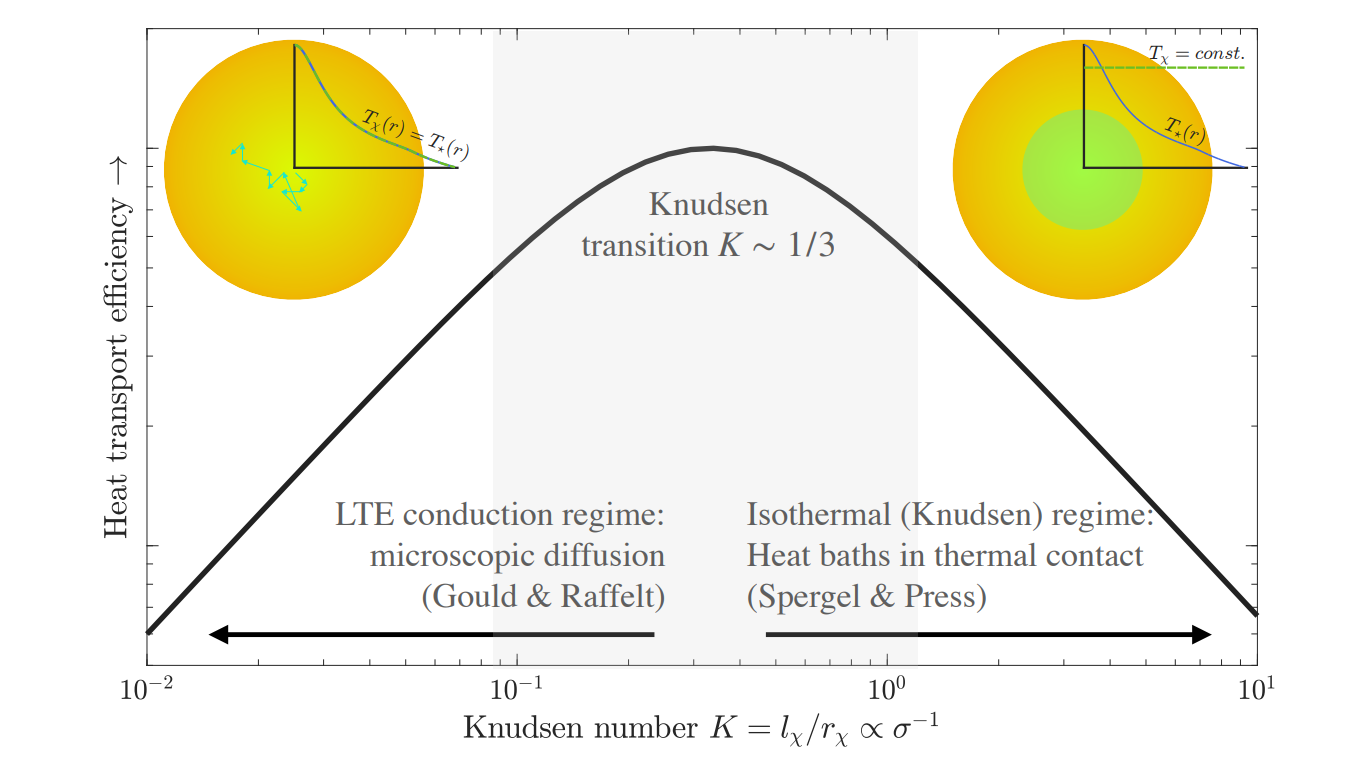
\includegraphics[width=.9\textwidth,height=.34\textheight]{figures/Regimi_conduzione_calore.png}
    \caption{Schematic diagram showing the two different regimes with their efficiency, from Banks et al \cite{Banks_2022}. As shown in the figure the most efficient regime is the one called \textit{Knudsen transition} and corresponds at about $K\sim \frac{1}{3}$.}
    \label{fig:Conductive_regimes}
\end{figure}

These two regimes correspond to the cases in which the DM could travel along all the structure, because his interaction length, and so the inverse of his cross-section,  is big enough to have almost no interactions; alternatively, the case in which the DM is confined because it has an enough big cross-section that bounds the DM to the SM particles. To have an idea of the orders of magnitude, in The Sun, the Knudsen transition corresponds to a cross-section, for spin-dependent and spin-independent interactions, of the order $\sigma_{SD}\sim 10^{-36} cm^2$, and $\sigma_{SI}\sim 10^{-37} cm^2$ \cite{Banks_2022}. It is possible to restrict the study to the Kundsen limit by looking at the latest experimental limits. The \textit{XENON1T} experiment narrowed the parameter space to $\sigma_{SI}=4.1\cdot 10^{-47}\, cm^2$ for mass around, and above, $m_{\chi}\sim 10\, \frac{GeV}{c^2}$ \cite{Xenon_2018}, and for the spin-dependent interaction the latest experimental limit is around $\sigma_{SD}\sim 10^{-41}\, cm^2$ \cite{Schumann_2019}.

\subsubsection{Isothermal conduction: the Kundsen limit}
Now, after focusing the attention of the study on the isothermal regime, it is possible to develop the specific transport equation by following Spergel and Press formalism \cite{SpergelPress_Cond, Banks_2022, DMSun}. 

The DM particles in principle, due to the few collisions with the star's elements and the very diluted density that prevent self-interactions, follow approximately the Maxwell-Boltzmann distribution, where, locally, the total energy of each particle is:
\begin{equation*}
    E_{\chi}(v_{\chi},r)=m_{\chi}\Big(\frac{v_{\chi}^2}{2}+ V(r)\Big)
\end{equation*}
Where $v_{\chi}$ is the DM velocity and V(r) is the gravitational potential inside the star. Moreover, we have to observe that the DM particles have an interaction length that allows them to orbit in a wide range of stellar radii, therefore it will not exist a unique star temperature ($T_{*}$); For each point,  the DM will tend to reach equilibrium with the local temperature without having the possibility to do it so we can not define a local equilibrium temperature for the entire structure. 
 Anyhow, like Spergel and Press demonstrate \cite{SpergelPress_Cond}, it's possible to solve the BCE in approximate form assuming that the DM sees a kind of averaged temperature $T_{\chi}$.
This means that the DM density inside the star follows the Boltzmann distribution:
\begin{equation*}
    n_{\chi}(r,t)=N_{\chi}(t)\frac{e^{\frac{-m_{\chi}V(r)}{k_B T_{\chi}}}}{\int_0^{R^{*}} 4 \pi r'^2 e^{\frac{-m_{\chi}V(r)}{k_B T_{\chi}}} dr'}
\end{equation*}
where $N_{\chi}(t)$ is the total number of particles captured at the time $t$. If we choose a sufficient fine time step in the simulation, it's possible to ignore the time dependence of the distribution.
We can moreover assume that the distribution is isotropic.

Therefore the DM has a phase space distribution, approximately, of this form:
\begin{equation}
\label{eq:DM_pahse_space}
    F_{\chi}(v_{\chi},r)=\Big(\frac{m_{\chi}}{2\pi k_{B}T_{\chi}}\Big)^{\frac{3}{2}}n_{\chi} e^{-\frac{m_{\chi}v^2_{\chi}}{2 k_B T_{\chi}}}
\end{equation}
on the other hand, the SM particles that compose the structure, due to local thermal equilibrium (LTE), follow locally the Maxwell-Boltzmann distribution, with the temperature $T_{*}(r)$, so their phase space distribution is:
\begin{equation*}
    F_{i}(v_i,r)=\Big(\frac{m_{i}}{2\pi k_{B}T_{*}}\Big)^{\frac{3}{2}}n_{i} e^{-\frac{m_i v^2_{i}}{2 k_B T_{*}}}
\end{equation*}
the index $i$ represents the distribution for each SM particle that composes the star.

Now if we apply the differential operator $D=\partial_t+\Vec{v}\cdot \Vec{\nabla}_r+ \Vec{g}(r)\cdot \Vec{\nabla}_v$ to the equation \ref{eq:DM_pahse_space}, we find that:
\begin{itemize}
    \item $\partial_t F_{\chi}=0$ because the distibution is stationary.
    \item $\Vec{v}_{\chi}\cdot \Vec{\nabla}_r F_{\chi}= -\frac{m_{\chi}V'(r)}{k_B T_{\chi}}F_{\chi}$
    \item $\Vec{g}(r)\cdot\Vec{\nabla}_v F_{\chi}=-V'(r)\frac{d}{dv}F_{\chi}=\frac{m_{\chi}V'(r)}{k_B T_{\chi}}F_{\chi}$
\end{itemize}
So under these assumptions, the BCE became a collision-less equation ($DF=0$). 
Given that, the DM does not add or remove energy from the structure but only transports it from the hotter zone to the cooler one. So by integrating over the whole structure, we have the condition\cite{DMSun}:
\begin{equation}
    \sum_i \int _0^{R_{*}} \epsilon_i(r,T_{\chi})4 \pi r^2 dr=0
\end{equation}
from which it is possible to find the DM temperature iteratively.

Despite the collision-less approximation, which is needed to have an estimation for $T_{\chi}$, the interaction between the DM and the SM particles plays an important role in the evolution of the star. During an interaction, the energy transferred to the DM is:
\begin{equation*}
    \Delta E= \frac{m_{\chi}}{2}(v_{\chi}'^2-v_{\chi}^2)
\end{equation*}
where the term superscript represents the velocity after the scattering. 

By definition, the energy transferred per unit time, species and volume is:
\begin{equation}
\label{eq:definition_epsilon}
    \epsilon_i\equiv \int d^3v_{\chi}F_{\chi}(v_{\chi},r)\int d^3v_i F_i(v_i,r)  \sigma \Delta E |v_{\chi}-v_i|
\end{equation}
In principle, the DM particle could scatter with a SM particle, which from now on we will represent with the $i$ index and an incident angle $\beta$. Now, if we make a Galilean transformation to a reference system (RS) where the $i$ particle is at rest the problem became bi-dimensional. In fact, in this RS  we have a cylindrical symmetry. In the center of mass system, we can treat the elastic scattering as a rotation. Hence boosting back the DM velocity after the scattering in the lab frame, subtracting the square of $v_{\chi}$ and weighting that with $\frac{m_{\chi}\sigma(\theta)}{2}$, we have that the transferred energy is a function of $v_{\chi},v_i,\beta,\theta_{cm}$, so averaging over the cosine of scattering angle, as in  \cite{SpergelPress_Cond}, we obtain:
\begin{equation}
    \Big< \Delta E (v_{\chi},v_i,\beta)\Big>=\frac{m_im_{\chi}}{(m_{\chi}+m_i)^2}(1-Q)[m_iv_i^2-m_{\chi}v_{\chi}^2+(m_{\chi}-m_i)v_{\chi}v_i\cos(\beta)]
\end{equation}
where
\begin{equation*}
    Q\equiv \frac{\int \sigma(\theta_{cm})\cos(\theta_{cm})d\cos(\theta_{cm})}{\int \sigma(\theta_{cm})d\cos(\theta_{cm})}
\end{equation*}
If we take the equation \ref{eq:definition_epsilon}, rewrite this in spherical coordinates, considering that the cross-section is energy independent, and using the average energy exchange, we have:
\begin{equation*}
\begin{split}
    \epsilon_i=\frac{8}{\pi}(C_iC_{\chi})^{\frac{3}{2}}\frac{m_im_{\chi}}{(m_{\chi}m_{i})^2}n_in_{\chi}(1-Q)\int_0^{2\pi} \sigma(\theta_{cm})d\cos(\theta_{cm}) \Bigg[\int_0^{\infty}v^2_{\chi}dv_{\chi} \\
    e^{-C_{\chi}v_{\chi}^2}\int_{v_{\chi}}^{\infty}v_i^2dv_i e^{C_iv_i^2}I_-+\int_0^{\infty}v^2_{\chi}dv_{\chi} e^{-C_{\chi}v_{\chi}^2}\int_{v_{i}}^{\infty}v_i^2dv_i e^{-C_iv_i^2}I_+\Bigg]  
\end{split}
\end{equation*}
where the integration is divided into two regions, $v_{\chi}\leq v_i$ and $v_{\chi}\geq v_i$ with:
\begin{equation*}
    I_{\pm}=\int_{z^{\pm}}^{v_{\chi}+v_i}[m_i v_i^2-m_{\chi}v_{\chi}^2+\frac{m_{\chi}-m_{i}}{2}(v_{\chi}^2)+v_i^2-z^2]\frac{z^2dz}{v_iv_{\chi}}
\end{equation*}
where the definition for the new variables are $z^2\equiv|\Vec{v}_{\chi}-\Vec{v}_i|^2$,$z^+\equiv v_i-v_{\chi}$, $z^-\equiv v_{\chi}-v_{i}$ and $C_{\chi/i}\equiv \frac{m_{\chi/i}}{2k_B T_{\chi/i}}$. Now integrating this last equation and defining the \textbf{conduction cross-section} as:
\begin{equation*}
    (1-Q)\int\sigma d\cos(\theta_{cm})\equiv \sigma_{cond}
\end{equation*} 
we obtain the energy transferred per unit time and volume:
\enfase{\begin{equation}
    \epsilon_i= 8\sqrt{\frac{2}{\pi}}n_{\chi}n_i\sigma_{cond}\frac{m_{\chi}m_{i}}{(m_{\chi}+m_i)^2}\Big(\frac{m_ik_BT_{\chi}+m_{\chi}k_BT_i}{m_i m_{\chi}}\Big)k_B(T_{i}-T{\chi})
\end{equation}}
It's important to notice that at maximum the conduction cross-section is the scattering cross-section, so the best case for the conduction effects is $\sigma_{cond}\simeq \sigma_{tot}$.
\section{State of the art for ADM in stars}
In this section, I will present the state of the art concerning the asymmetric dark matter in stars, focusing the attention in particular on ADM that corresponds to the case in which it introduces a new energy transport channel in the Knudsen limit, previously introduced.

%appendices
\pagestyle{plain}
\clearpage
\appendix
\pagenumbering{Roman}

%appendix section
\section{Analytic theory of DM capture}
\label{App:capture}
\section{DM scale height inside the star}
\label{App:DM_Scale_height}
Following the notation in reference \cite{SpergelPress_Cond}, and assuming that the captured DM is in thermal equilibrium with the star, it populates a small core region where it's roughly valid the equation:
\begin{equation*}
\frac{3}{2}k_B T_c=m_{\chi}V(r_{\chi})
\end{equation*}
where $T_c$ is the central temperature of the star. Now, making a second approximation, we can consider this star region as an equal density region at $\rho_c$, obtaining that:
\begin{equation*}
    V(r)\simeq \frac{2\pi}{3}G\rho_cr^2
\end{equation*}
so these two equations give:
\begin{equation*}
    r_{\chi}=\Big(\frac{9}{4\pi}\frac{k_BT_c}{G\rho_c m_{\chi}}\Big)^{\frac{1}{2}}
\end{equation*}

This scale height is useful to have a first comprehension of the DM distribution inside the star. It's possible to define the DM mean free path as:
\begin{equation*}
    l_{\chi}=\frac{1}{\sum n_{i}\sigma_{i}}
\end{equation*}
Where it was considered the presence of different nuclei inside the star. Therefore we could compare the dimension of these two variables and define two apposite regimes, one, where the mean free path is much smaller than the scale height of DM core and the other one where the DM core scale height is much smaller than the mean free path. In the first one, which is called also the local thermal equilibrium regime, the DM makes many interactions inside the core reaching the equilibrium whit the stellar structure locally,  in the second, the DM is practically free, so it travels along all the stellar structure without reaching that.

%bibliography
\clearpage
\pagenumbering{roman}
\addcontentsline{toc}{section}{\refname} % Manually add the bibliography to the table of contents
\bibliographystyle{plainurl}
\bibliography{sample}

%acknowledgments
\pagestyle{empty}
\clearpage
% Acknowledgments
\section*{Acknowledgments}
I would like to express my sincere gratitude to...


% Blank page
\newpage

\mbox{}

\end{document}